\documentclass{beamer}

\mode<presentation> {

%\usetheme{default}
%\usetheme{AnnArbor}
%\usetheme{Antibes}
%\usetheme{Bergen}
%\usetheme{Berkeley}
%\usetheme{Berlin}
%\usetheme{Boadilla}
%\usetheme{CambridgeUS}
%\usetheme{Copenhagen}
%\usetheme{Darmstadt}
%\usetheme{Dresden}
%\usetheme{Frankfurt}
%\usetheme{Goettingen}
%\usetheme{Hannover}
%\usetheme{Ilmenau}
%\usetheme{JuanLesPins}
%\usetheme{Luebeck}
\usetheme{Madrid}
%\usetheme{Malmoe}
%\usetheme{Marburg}
%\usetheme{Montpellier}
%\usetheme{PaloAlto}
%\usetheme{Pittsburgh}
%\usetheme{Rochester}
%\usetheme{Singapore}
%\usetheme{Szeged}
%\usetheme{Warsaw}


%\usecolortheme{albatross}
%\usecolortheme{beaver}
%\usecolortheme{beetle}
%\usecolortheme{crane}
%\usecolortheme{dolphin}
%\usecolortheme{dove}
%\usecolortheme{fly}
%\usecolortheme{lily}
%\usecolortheme{orchid}
%\usecolortheme{rose}
%\usecolortheme{seagull}
%\usecolortheme{seahorse}
%\usecolortheme{whale}
%\usecolortheme{wolverine}

%\setbeamertemplate{footline} % To remove the footer line in all slides uncomment this line
%\setbeamertemplate{footline}[page number] % To replace the footer line in all slides with a simple slide count uncomment this line

%\setbeamertemplate{navigation symbols}{} % To remove the navigation symbols from the bottom of all slides uncomment this line
}

\usepackage{graphicx} % Allows including images
\usepackage{booktabs} % Allows the use of \toprule, \midrule and \bottomrule in tables
\usepackage{amsfonts}
\usepackage{mathrsfs}
\usepackage{amsmath,amssymb,graphicx, bm}

%----------------------------------------------------------------------------------------
%	TITLE PAGE
%----------------------------------------------------------------------------------------

\title["6.3"]{6.3: Unit Roots in Time Series Models} 

\author{Taylor} 
\institute[UVA] 
{
University of Virginia \\
\medskip
\textit{} 
}
\date{} 

\begin{document}
%----------------------------------------------------------------------------------------

\begin{frame}
\titlepage 
\end{frame}

%----------------------------------------------------------------------------------------

\begin{frame}
\frametitle{Motivation}

``...a root near $1$ of the autoregressive polynomial suggests that the data
should be differenced before fitting an ARMA model, whereas a root near $1$ of
the moving-average polynomial indicates that the data were overdifferenced."
\newline

% Unit root tests are used a lot of econometrics. For example in ``statistical arbitrage" or ``pairs trading" a portfolio/linear-combination of assets is constructed that is ideally stationary (no unit-root). 


\end{frame}

%----------------------------------------------------------------------------------------

\begin{frame}
\frametitle{Testing non-stationarity}

Assume an AR(1) model: $X_t - \mu = \phi_1( X_{t-1} - \mu) + Z_t$. 
\newline

We want to test $H_0: \phi_1 = 1$. Under the null hypothesis, our time series is a random walk (not stationary). 
\newline

The standard large sample asymptotic distributions for our estimators of $\phi_1$ only apply when $|\phi_1| < 1$.
\newline

Q: What do we do?

\end{frame}

%----------------------------------------------------------------------------------------

\begin{frame}
\frametitle{Test: $H_0: \phi_1 = 1$}

A: We take the difference!

Our AR(1) model: $X_t - \mu = \phi_1( X_{t-1} - \mu) + Z_t$ \\
becomes:

\begin{align*}
\triangledown X_t &=  \mu + \phi_1( X_{t-1} - \mu) + Z_t - X_{t-1} \\
&= \mu(1 - \phi_1) + ( \phi_1 - 1) X_{t-1} + Z_t \\
&= \phi^*_0 + \phi^*_1 X_{t-1} + Z_t
\end{align*}

Now we test the null hypothesis: $H_0: \phi^*_1 = 0$.

\end{frame}

%----------------------------------------------------------------------------------------

\begin{frame}
\frametitle{Test: $H_0: \phi_1 = 1$}

Even though we test the null hypothesis: $H_0: \phi^*_1 = 0$, we estimate the full regression model
\[
\triangledown X_t = \phi^*_0 + \phi^*_1 X_{t-1} + Z_t
\]

We get the familiar t-test statistic (only it doesn't follow a t-distribution under the null this time)

\[
\hat{\tau}_{\mu} = \frac{\hat{\phi}_1^* }{ \sqrt{\frac{S^2}{\sum_{t=2}^n(X_{t-1}-\bar{X})^2 } } }
\]

where $S^2 = \sum_{t=2}^n (\triangledown X_t - \hat{\phi}^*_0 - \hat{\phi}_1^* X_{t-1})^2/(n-1 - 2)$

\end{frame}

%----------------------------------------------------------------------------------------

\begin{frame}
\frametitle{Test: $H_0: \phi_1 = 1$}

Dickey and Fuller derived the asymptotic distribution of this quantity. 
\[
\hat{\tau}_{\mu} = \frac{\hat{\phi}_1^* }{ \sqrt{\frac{S^2}{\sum_{t=2}^n(X_{t-1}-\bar{X})^2 } } }
\]

where $S^2 = \sum_{t=2}^n (\triangledown X_t - \hat{\phi}^*_0 - \hat{\phi}_1^* X_{t-1})^2/(n-3)$
\newline

You reject the null when this thing is small. The $0.01$, $0.05$, and $0.10$ quantiles of the limit
distribution of $\hat{\tau}_{\mu}$ are $-3.43$, $-2.86$, and $-2.57$ (see Table 8.5.2 of Fuller 1976 or R code printout)
\newline

See 6.3.R

\end{frame}
\begin{frame}
\frametitle{Example}

When you assume the true model is a higher order AR process, the test is called the *augmented* Dickey-Fuller test.
\newline

A homework question asks you to show that the AR($p$) model 
\[
X_t - \mu  = \phi_1 (X_{t-1} - \mu ) + \cdots + \phi_p(X_{t-p} - \mu ) + Z_t
\]
can be written as
\[
\triangledown X_t = \phi_0^* + \phi_1^* X_{t-1} + \phi_2^*\triangledown X_{t-1} + \cdots + \phi_p^*\triangledown X_{t-p+1} + Z_t
\]

\end{frame}

%----------------------------------------------------------------------------------------

\begin{frame}[fragile]
\frametitle{Example 1}

Recall that the null is non-stationary with a unit root, and the test is a ``left-tailed" test. We generate data with a unit root, so the data shouldn't reject the hypothesis most of the time. 
\begin{verbatim}
library(urca)

# generate data from an arima(1,1,0) model
fakeData <- arima.sim(model = list(ar=c(.9), order = c(1,1,0)), n=100)
plot.ts(fakeData)
summary(ur.df(fakeData, type = "drift", lags=1)) # regular dickey fuller
summary(ur.df(fakeData, type = "drift", lags=3)) # augmented dickey fuller for AR(3)
\end{verbatim}

\end{frame}

%----------------------------------------------------------------------------------------

\begin{frame}[fragile]
\frametitle{Example 2}

Let's pretend you've bought one nasdaq share and sold short one S\&P. This looks like a nice portfolio because it appears to trend up, and you don't have to re-balance your weights (it's always 1 to 1, so no transaction costs). 

\begin{verbatim}
getSymbols(c("SPY","QQQQ"), src = "google")
xt <- SPY$SPY.Close - QQQQ$QQQQ.Close
xt <- xt[500:2714] # :)
plot.ts(xt)
\end{verbatim}

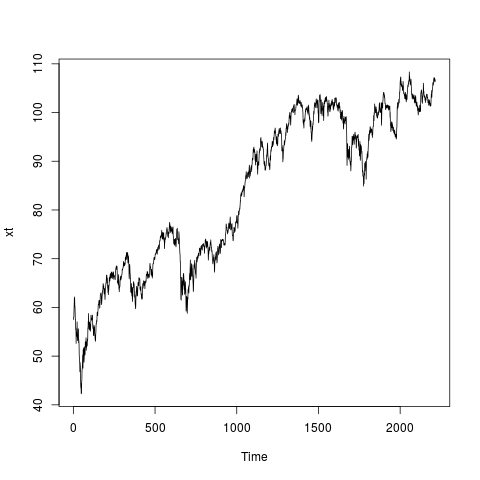
\includegraphics[width=50mm]{/home/taylor/UVa/all_teaching/4170_slides/6/6.3/pics/Rplot}

\end{frame}

%----------------------------------------------------------------------------------------

\begin{frame}[fragile]
\frametitle{Example 2: Is there Mean-Reversion?}

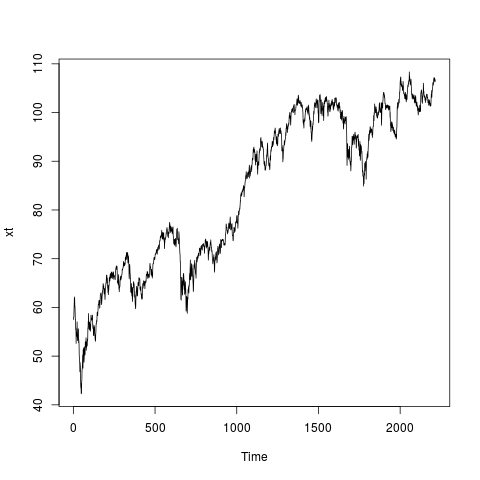
\includegraphics[width=50mm]{/home/taylor/UVa/all_teaching/4170_slides/6/6.3/pics/Rplot}

This $X_t$ doesn't look stationary, but is it a ``stochastic trend"
\[
\phi(B)(1-B)(X_t-\mu t) = \theta(B)Z_t
\]
or a ``deterministic trend"
\[
\phi(B)(X_t - [\beta_0 + \beta_1 t]) = \theta(B) Z_t?
\]
Note that we can write the last one as a regression plus ARMA error if (if $\phi(z)$ is causal) .
\end{frame}


%----------------------------------------------------------------------------------------

\begin{frame}[fragile]
\frametitle{Example}

\begin{verbatim}
myTest <- ur.df(xt, "trend") # note "trend"
summary(myTest)

Value of test-statistic is: -3.0016 4.9831 4.616 

Critical values for test statistics: 
      1pct  5pct 10pct
tau3 -3.96 -3.41 -3.12
phi2  6.09  4.68  4.03
phi3  8.27  6.25  5.34
\end{verbatim}


\end{frame}

%----------------------------------------------------------------------------------------

\begin{frame}[fragile]
\frametitle{Unit Roots in the MA polynomial}

Why are unit roots bad in the MA polynomial?
\newline

Reason 1: if $\phi(B) X_t = \theta(B) Z_t$ is the true model, a causal and invertible ARMA(p,q), then $\triangledown X_t$ is a non-invertible ARMA(p,q+1).

\begin{align*}
\phi(B) \triangledown X_t &= \phi(B)X_t - \phi(B)X_{t-1}  \\
&= \theta(B)Z_t - \theta(B) Z_{t-1} \\
&= \theta(B)(1 - B)Z_t
\end{align*}

...test of overdifferencing...
\end{frame}

%----------------------------------------------------------------------------------------

\begin{frame}[fragile]
\frametitle{Unit Roots in the MA polynomial}

Reason 2: Which model is correct? Consider again the difference between a stochastic trend, and a deterministic trend. 

\[
\triangledown^k X_t  = a + V_t
\]
or
\[
X_t = c_0 + c_1t + \cdots + c_k t^k + W_t
\]
The former has unit roots, while the latter has none.

\end{frame}

%----------------------------------------------------------------------------------------

\begin{frame}[fragile]
\frametitle{Unit Roots in the MA polynomial}

Simplify by setting $k=1$ which is what happens most of the time in financial time series anyways
\[
X_t = c + X_{t-1} + Z_t \iff \triangledown X_t = c + Z_t
\]
and
\[
X_t = a + c t + Z_t \iff \triangledown X_t = c +  Z_t - Z_{t-1}
\]
If you run one simulation for each, they look very similar! However, the second one has a unit root. 
\newline

Watch out for overdifferencing!
\end{frame}






\end{document} 